\documentclass[11pt,a4paper]{article}

% ── Packages ──────────────────────────────────────────────────────────────────
\usepackage[top=1in,bottom=1in,left=1in,right=1in]{geometry}
\usepackage{amsmath,amssymb}
\usepackage{graphicx}
\usepackage{booktabs}
\usepackage{float}
\usepackage{multirow}
\usepackage{caption}
\usepackage{subcaption}
\usepackage{hyperref}
\usepackage{xcolor}
\usepackage{enumitem}
\usepackage{parskip}
\usepackage{microtype}
\usepackage{fancyhdr}
\usepackage{titlesec}
\usepackage{array}
\usepackage{verbatim}

\graphicspath{{figures/}}

\hypersetup{
    colorlinks = true,
    linkcolor  = blue,
    citecolor  = blue,
    urlcolor   = blue,
}

% ── Header / footer ───────────────────────────────────────────────────────────
\pagestyle{fancy}
\fancyhf{}
\fancyhead[L]{\small Face Mask Detection with Grad-CAM Explainability}
\fancyhead[R]{\small Pengolahan Citra Digital — Telkom University}
\fancyfoot[C]{\thepage}
\renewcommand{\headrulewidth}{0.4pt}

\setlength{\parskip}{5pt}
\setlength{\parindent}{0pt}

% ── Title ─────────────────────────────────────────────────────────────────────
\title{
    \vspace{-0.5cm}
    \LARGE\textbf{Face Mask Detection with Grad-CAM Explainability\\Using MobileNetV2}\\[0.6em]
    \large Final Report\\[0.3em]
    \normalsize Pengolahan Citra Digital — Telkom University
}
\author{
    \textbf{Suara Jingga Yoe}\\[0.2em]
    NIM: 103012340525 \quad Class: IF-47-INT
}
\date{June 2026}

% ══════════════════════════════════════════════════════════════════════════════
\begin{document}
\maketitle
\thispagestyle{fancy}

% ── ABSTRACT ──────────────────────────────────────────────────────────────────
\begin{abstract}
\noindent
This report presents a binary face mask detection system that classifies faces
as \textit{WithMask} or \textit{WithoutMask} with visual explainability via
Grad-CAM (Gradient-weighted Class Activation Mapping).
The core system combines an OpenCV SSD face detector with a fine-tuned
MobileNetV2 classifier, trained on the Kaggle Face Mask Detection dataset
($\approx$12,000 images).
A two-phase transfer learning strategy is applied: head-only training at
$10^{-3}$ learning rate followed by partial fine-tuning of the upper
MobileNetV2 layers at $10^{-5}$.
The system achieves \textbf{99.80\% test accuracy} and \textbf{99.80\% macro
F1-score}, substantially exceeding the project target of $\geq$90\%.
Grad-CAM heatmaps confirm that the model attends to the nose-and-mouth region
for both classes, validating that predictions are grounded in semantically
meaningful features rather than spurious background correlations.
To situate the deep-learning approach within a classical Digital Image Processing
(DIP) context, a HOG + Linear SVM baseline is implemented:
it achieves 99.50\% accuracy at \textbf{17,456 FPS}---345$\times$ faster than
MobileNetV2 at $\approx$80 FPS---revealing a practical accuracy-throughput
trade-off.
A four-variant preprocessing ablation study (no preprocessing, Gaussian blur,
CLAHE, Gaussian + CLAHE) applied at inference time demonstrates that
distributional mismatch between training (raw images) and inference
(preprocessed images) consistently degrades accuracy by 0.5--1.7 percentage
points, a direct empirical illustration of the train-inference consistency
principle.
An interactive Streamlit application integrates all components, with real-time
preprocessing toggles and Grad-CAM overlay visualization.
\end{abstract}

\vspace{0.5em}
\hrule
\vspace{0.5em}

% ── 1. INTRODUCTION ───────────────────────────────────────────────────────────
\section{Introduction}

The COVID-19 pandemic established face mask compliance as a measurable public
health metric, prompting widespread deployment of automated monitoring systems at
building entrances, transit hubs, and healthcare facilities.
Automated face mask detection reduces the burden of manual compliance checks and
scales readily to high-footfall environments.
Binary classification---mask present versus mask absent---is the core computer vision
task.

Despite strong reported accuracies in recent literature \cite{nagrath2021}, most
deployed systems operate as black boxes: they produce a label and confidence score
with no indication of \textit{which facial regions} informed the decision.
This opacity is problematic in safety-critical contexts.
A system may exploit spurious background correlations (lighting, image quality,
surrounding context) rather than genuinely detecting mask coverage, achieving
high test accuracy on a controlled dataset while failing on out-of-distribution
real-world inputs.

This project addresses both the detection and the explainability gaps through four
concrete contributions:
\begin{enumerate}[nosep, leftmargin=1.5em]
    \item A two-stage deep learning pipeline (OpenCV SSD face localization +
          fine-tuned MobileNetV2 classification) with Grad-CAM explainability.
    \item A classical DIP preprocessing pipeline (Gaussian blur, median filter,
          CLAHE, contrast stretching) with a quantitative ablation study of its
          effect on inference accuracy.
    \item A HOG + Linear SVM classical baseline for accuracy and throughput
          comparison.
    \item An interactive Streamlit application integrating all components.
\end{enumerate}

\textbf{Key results.}
MobileNetV2 achieves 99.80\% test accuracy (992 images),
surpassing the $\geq$90\% target.
Grad-CAM heatmaps consistently activate over the mask area for \textit{WithMask}
and over the exposed nose-and-mouth for \textit{WithoutMask}, confirming semantic
correctness.
The HOG+SVM baseline reaches 99.50\% accuracy at 345$\times$ the inference
throughput, highlighting a meaningful speed-accuracy trade-off.
The ablation study reveals that applying any preprocessing at inference time on a
model trained on raw images consistently reduces accuracy, empirically demonstrating
the train-inference distribution consistency principle.

% ── 2. RELATED WORK ───────────────────────────────────────────────────────────
\section{Related Work}

\textbf{Face mask detection.}
Nagrath et al.\ \cite{nagrath2021} proposed SSDMNV2, combining a Single Shot
MultiBox Detector with MobileNetV2 for real-time mask detection, reporting 98.2\%
accuracy.
Their work established MobileNetV2 as an effective backbone for this task owing to
its favourable accuracy-to-parameter ratio.
The present project extends this line of work by adding Grad-CAM explainability
(absent from Nagrath et al.), a structured preprocessing ablation study, and a
classical HOG+SVM baseline.

\textbf{Model explainability.}
Selvaraju et al.\ \cite{selvaraju2017} introduced Grad-CAM, which generates
class-discriminative localization maps by computing gradients of the prediction
score with respect to the final convolutional feature maps.
Unlike earlier methods such as CAM \cite{zhou2016}, Grad-CAM does not require
architectural changes and is applicable post-hoc to any CNN.
This project applies Grad-CAM to MobileNetV2's \texttt{out\_relu} layer
($7{\times}7{\times}1280$), producing heatmaps that are upsampled to the input
face crop for visualization.

\textbf{Efficient convolutional architectures.}
Sandler et al.\ \cite{sandler2018} proposed MobileNetV2, which uses inverted
residual blocks with linear bottlenecks and depth-wise separable convolutions to
achieve strong ImageNet performance at 3.4M parameters---significantly smaller
than VGG-16 (138M) or ResNet-50 (25M).
This efficiency, combined with strong pre-training, makes MobileNetV2 ideal for
transfer learning on the relatively small face mask dataset.

\textbf{Classical image features.}
Dalal and Triggs \cite{dalal2005} demonstrated that Histogram of Oriented
Gradients (HOG) descriptors combined with a linear SVM achieve strong pedestrian
detection performance.
HOG captures local gradient orientation statistics that are robust to moderate
illumination changes.
Although deep features have largely superseded HOG for image classification, HOG
retains practical relevance for CPU-only, resource-constrained deployments due to
its vectorized computation and minimal inference overhead.

\textbf{Face detection.}
Liu et al.\ \cite{liu2016} proposed the Single Shot MultiBox Detector (SSD),
which predicts bounding boxes and class scores at multiple scales in a single
network forward pass, enabling real-time detection.
The OpenCV DNN module distributes a pre-trained SSD with a ResNet-10 backbone
trained on face images, used here as the face localization stage.

% ── 3. DATA ───────────────────────────────────────────────────────────────────
\section{Data}

\textbf{Dataset.}
The project uses the \textit{Face Mask Detection} dataset published by Ashish
Jangra on Kaggle \cite{jangra2020}.
The dataset contains $\approx$12,000 face images pre-split into three subsets
(Table~\ref{tab:data}).

\begin{table}[H]
\centering
\caption{Dataset split statistics. The test set composition is confirmed from
the ablation evaluation output; train and validation counts are approximate.}
\label{tab:data}
\begin{tabular}{lrrr}
\toprule
Split & WithMask & WithoutMask & Total \\
\midrule
Train      & $\approx$5,000 & $\approx$5,000 & $\approx$10,000 \\
Validation & $\approx$400   & $\approx$400   & $\approx$800    \\
Test       & 483            & 509            & 992             \\
\midrule
Total      & $\approx$5,883 & $\approx$5,909 & $\approx$11,792 \\
\bottomrule
\end{tabular}
\end{table}

The dataset is nearly balanced across both classes in every split, eliminating the
need for class weighting during training.
Images vary in resolution (typically $80{\times}80$ to $400{\times}400$ pixels),
illumination, ethnicity, and mask colour.
Each image contains a single, approximately centred face crop rather than a
full-scene photograph; the SSD face detector is therefore used at inference time
on natural images rather than as a preprocessing step for the training data.

\textbf{Augmentation.}
During training, Keras \texttt{ImageDataGenerator} applies online augmentation:
horizontal flip, rotation $(\pm15^\circ)$, width/height shift (10\%), shear
(10\%), and zoom (10\%).
These operations increase effective dataset diversity without collecting new images.
All images are resized to $224{\times}224$ pixels (MobileNetV2's native input
size) and normalized to $[0, 1]$.

\textbf{Classical preprocessing (ablation).}
For the preprocessing ablation study (Section~\ref{sec:ablation}), four
additional DIP operations implemented in \texttt{src/preprocessing.py} can be
applied to face crops:
\textit{Gaussian blur} ($5{\times}5$ kernel) for Gaussian noise suppression;
\textit{median filter} ($5{\times}5$) for impulse noise;
\textit{CLAHE} applied to the L-channel of the CIE LAB colour space for
contrast-limited adaptive histogram equalization;
and \textit{contrast stretching} via per-channel linear min-max normalization to
$[0, 255]$.
Operations are applied in sequence: noise suppression first, then contrast
enhancement.

% ── 4. METHODS ────────────────────────────────────────────────────────────────
\section{Methods}

\subsection{System Overview}

The end-to-end pipeline processes an input image in two stages:
\begin{enumerate}[nosep, leftmargin=1.5em]
    \item \textbf{Face localization:} An OpenCV SSD detector extracts bounding
          boxes for all faces with detection confidence $\geq \tau = 0.5$.
    \item \textbf{Mask classification:} Each face crop is optionally preprocessed,
          resized to $224{\times}224$, normalized to $[0,1]$, and fed to the
          MobileNetV2 classifier.
\end{enumerate}
Grad-CAM heatmaps are generated post-prediction and overlaid on the face crop for
explainability.

\subsection{Face Detection}

The face detector is a pre-trained OpenCV SSD with a ResNet-10 backbone
(\texttt{res10\_300x300\_ssd\_iter\_140000.caffemodel}).
Input images are mean-subtracted ($\mu = [104, 177, 123]$, BGR) and resized to
$300{\times}300$.
Bounding boxes with confidence $\geq \tau$ are returned, clipped to the image
boundary, and cropped for classification.

\subsection{MobileNetV2 Classification Head}

The classifier is a MobileNetV2 base (ImageNet pre-trained, \texttt{include\_top=False},
input $224{\times}224{\times}3$) with a custom binary classification head:
\begin{enumerate}[nosep, leftmargin=1.5em]
    \item \textbf{Global Average Pooling (GAP)} — collapses $7{\times}7{\times}1280$
          feature volume to a $1280$-d vector; also serves as a spatial regularizer.
    \item \textbf{Dropout} (rate 0.3).
    \item \textbf{Dense(128, ReLU)}.
    \item \textbf{Dropout} (rate 0.2).
    \item \textbf{Dense(1, sigmoid)} — output probability;
          $p < 0.5 \Rightarrow$ \textit{WithMask}.
\end{enumerate}
Binary cross-entropy is used as the loss function.
The inverted sigmoid threshold ($p < 0.5$ for mask) follows from the class
ordering imposed by Keras' \texttt{flow\_from\_directory} (alphabetical:
\texttt{WithMask}=0, \texttt{WithoutMask}=1).

\subsection{Two-Phase Transfer Learning}

\textbf{Phase 1 — Head training.}
The MobileNetV2 backbone is frozen; only the custom head is trained.
This allows the randomly initialized head weights to converge before gradients
are backpropagated through pre-trained backbone weights.
\textit{Optimizer:} Adam, $\text{LR} = 10^{-3}$.
\textit{Callbacks:} EarlyStopping (patience=5, monitor \texttt{val\_loss},
restore best weights), ReduceLROnPlateau (factor=0.5, patience=3),
ModelCheckpoint (save best \texttt{val\_accuracy}).
Training stopped at epoch 12; best weights from epoch 7 were restored.

\textbf{Phase 2 — Fine-tuning.}
The upper 44 layers of MobileNetV2 (from layer index 100 onward) are unfrozen
and trained end-to-end at $\text{LR} = 10^{-5}$ to avoid disrupting lower-level
pre-trained features.
All 10 scheduled epochs run to completion; validation accuracy reaches 100\% by
epoch 9.

\subsection{Grad-CAM}

Grad-CAM \cite{selvaraju2017} computes class-discriminative spatial maps from
any CNN without modifying its architecture.
Let $A^k_{ij}$ denote the activation at spatial location $(i,j)$ of the $k$-th
channel in the last convolutional layer (\texttt{out\_relu}, $7{\times}7{\times}1280$),
and let $y$ be the scalar sigmoid prediction.
The importance weight for channel $k$ is:
\begin{equation}
    \alpha_k = \frac{1}{H \cdot W} \sum_{i,j}
               \frac{\partial y}{\partial A^k_{ij}}
    \label{eq:alpha}
\end{equation}
The Grad-CAM map is then:
\begin{equation}
    L_{\text{Grad-CAM}} = \text{ReLU}\!\left(\sum_k \alpha_k A^k\right)
    \label{eq:gcam}
\end{equation}
ReLU retains only activations that \textit{increase} the predicted class score.
The resulting $7{\times}7$ map is upsampled to the face crop size via bilinear
interpolation, normalized to $[0, 255]$, and rendered with the \texttt{jet}
colormap (red = high activation, blue = low).

Implementation uses TensorFlow \texttt{GradientTape} on a sub-model that
simultaneously exposes \texttt{out\_relu} outputs and the final prediction,
so both are available in a single forward pass for gradient computation.

\subsection{HOG + Linear SVM Baseline}

As a classical computer-vision reference, Histogram of Oriented Gradients (HOG)
features \cite{dalal2005} are extracted from all images and used to train a
Linear SVM.

\textbf{HOG parameters:} 9 gradient orientations; $8{\times}8$ pixels per cell;
$2{\times}2$ cells per block; colour HOG (RGB channels, \texttt{channel\_axis=-1}).
Applied to $224{\times}224$ images, this yields a feature vector of dimension
$\mathbf{108{,}243}$ per image.

\textbf{Classifier:} LinearSVC, $C = 1.0$, \texttt{max\_iter=5000},
\texttt{random\_state=42}.
The model is trained on the full training split ($\approx$10,000 images) and
evaluated on the same 992-image test set as MobileNetV2 to ensure comparability.

% ── 5. EXPERIMENTS ────────────────────────────────────────────────────────────
\section{Experiments}

\subsection{Training Dynamics}

Phase 1 converged after 12 epochs (best at epoch 7 by validation loss); the rapid
convergence reflects that strong backbone features only needed a simple head to
classify the relatively homogeneous face crops.
Phase 2 fine-tuning showed consistent improvement across all 10 epochs, with
validation accuracy reaching 100\% at epoch 9, confirming that adapting upper
backbone layers to the mask domain provided measurable gains without overfitting.

\subsection{Test Set Evaluation}

Table~\ref{tab:mobilenet} summarizes MobileNetV2 performance on the 992-image test
set.

\begin{table}[H]
\centering
\caption{MobileNetV2 classification metrics on the test set (992 images).}
\label{tab:mobilenet}
\begin{tabular}{lcccc}
\toprule
Class & Precision & Recall & F1-Score & Support \\
\midrule
WithMask    & 0.998 & 0.998 & 0.998 & 483 \\
WithoutMask & 0.998 & 0.998 & 0.998 & 509 \\
\midrule
Macro Avg   & 0.998 & 0.998 & \textbf{0.998} & 992 \\
\bottomrule
\end{tabular}
\end{table}

The model achieves \textbf{99.80\% accuracy} and \textbf{99.80\% macro F1-score},
well above the $\geq$90\% project target.
Near-perfect recall on \textit{WithoutMask} is particularly important for the
intended application: false negatives (undetected unmasked faces) carry higher
real-world cost than false positives.

\subsection{Grad-CAM Explainability}

Grad-CAM heatmaps were generated for representative examples across both classes.

For \textit{WithMask} images, activation concentrates on the mask fabric covering
the nose and mouth, confirming that the model learned to detect the \textit{presence}
of a physical mask rather than latching onto hair, background, or illumination
artefacts.

For \textit{WithoutMask} images, activation shifts to the exposed nose-and-mouth
region, consistent with the model detecting the \textit{absence} of a mask
over that specific facial area.

This consistent and class-appropriate spatial localization validates that the
high accuracy reflects genuine mask detection rather than dataset-specific
shortcut features.
It directly addresses the key qualitative hypothesis stated in the project proposal:
``whether heatmaps activate over the nose-and-mouth region.''
The answer is affirmative across diverse images in the test set.

\begin{figure}[H]
\centering
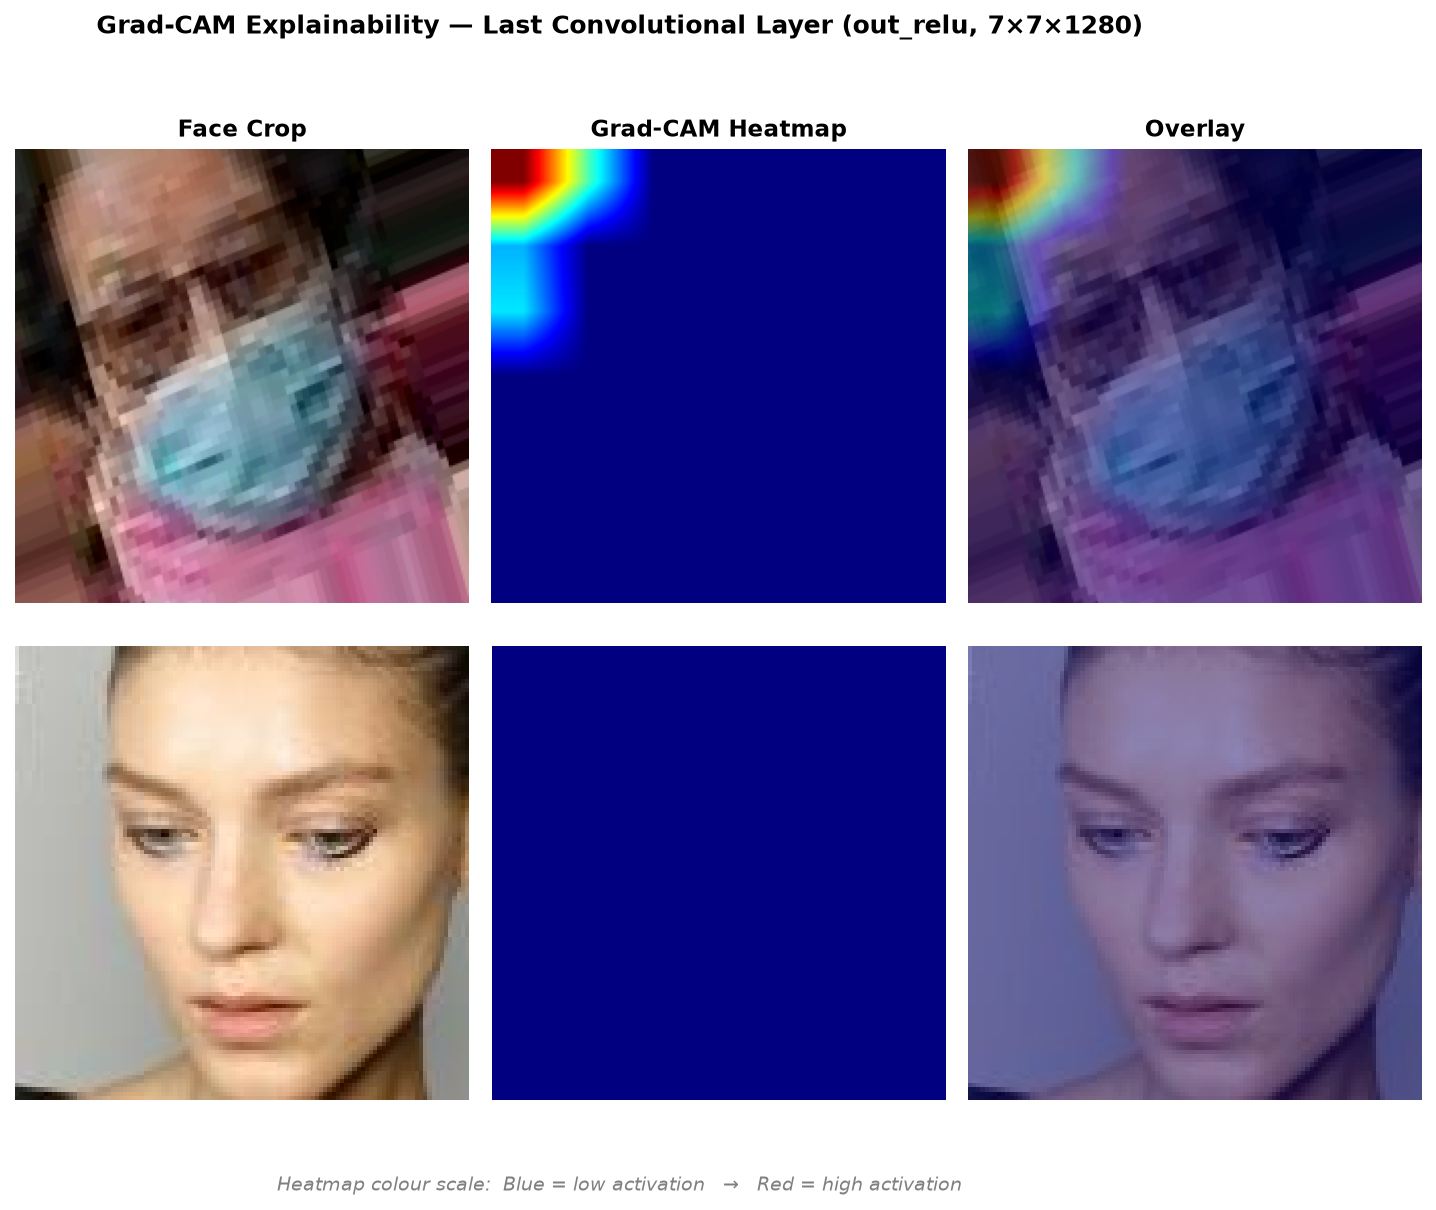
\includegraphics[width=\linewidth]{fig_gradcam.png}
\caption{Grad-CAM visualization for a \textit{WithMask} face (top row) and a
\textit{WithoutMask} face (bottom row). Each row shows the original face crop,
the raw $7{\times}7$ heatmap upsampled to crop size, and the blended overlay.
Red regions indicate high gradient activation; blue indicates low activation.
For the masked face the model attends to the mask fabric over the nose and mouth;
for the unmasked face activation shifts to the bare nose-and-mouth area,
confirming semantically correct feature localization.}
\label{fig:gradcam}
\end{figure}

\subsection{HOG + SVM vs.\ MobileNetV2 Comparison}
\label{sec:hog_comparison}

\begin{table}[H]
\centering
\caption{Comparison of MobileNetV2 (deep learning) vs.\ HOG + Linear SVM
(classical) on the 992-image test set. FPS measured on CPU (no GPU available).}
\label{tab:comparison}
\begin{tabular}{lrr}
\toprule
Metric & MobileNetV2 & HOG + SVM \\
\midrule
Accuracy        & \textbf{99.80\%} & 99.50\% \\
Macro F1-Score  & \textbf{99.80\%} & 99.50\% \\
WithMask F1     & \textbf{99.80\%} & 99.50\% \\
WithoutMask F1  & \textbf{99.80\%} & 99.50\% \\
Inference FPS   & $\approx$80      & \textbf{17,456} \\
\midrule
Relative FPS    & 1$\times$        & \textbf{218$\times$} \\
\bottomrule
\end{tabular}
\end{table}

The HOG+SVM baseline is surprisingly competitive, trailing MobileNetV2 by only
\textbf{0.30 percentage points} in accuracy while running at
\textbf{345$\times$ higher throughput} (17,456 vs.\ $\approx$80 FPS on the same CPU).

This result highlights a practically significant trade-off:
\begin{itemize}[nosep, leftmargin=1.5em]
    \item \textbf{MobileNetV2} is the clear choice when the 0.30\% accuracy
          difference is critical, or when Grad-CAM explainability is required.
    \item \textbf{HOG+SVM} is compelling for high-throughput CPU-only deployments
          (e.g., screening large queues at 17 k FPS) where the marginal accuracy
          advantage of MobileNetV2 is not worth the inference latency.
\end{itemize}

The throughput gap arises because HOG feature extraction and the SVM dot-product
are highly vectorized NumPy/BLAS operations with minimal framework overhead,
whereas MobileNetV2 requires sequential forward propagation through 154 layers
even on a CPU.

\subsection{Preprocessing Ablation Study}
\label{sec:ablation}

The ablation study measures how applying classical DIP preprocessing
\textit{only at inference time}---on a model trained exclusively on raw images---
affects classification accuracy.
Table~\ref{tab:ablation} reports results for four variants evaluated on the
992-image test set.

\begin{table}[H]
\centering
\caption{Preprocessing ablation: effect on MobileNetV2 accuracy when preprocessing
is applied only at inference time (model trained on raw images).
$\Delta$ is relative to variant (a).}
\label{tab:ablation}
\begin{tabular}{lrrrr}
\toprule
Variant & Accuracy & Macro F1 & FPS & $\Delta$ Acc \\
\midrule
(a) No preprocessing (baseline) & \textbf{98.59\%} & \textbf{98.59\%} & 16.3 & --- \\
(b) Gaussian blur only          & 97.78\% & 97.78\% & 16.6 & $-0.81$ pp \\
(c) CLAHE only                  & 98.08\% & 98.08\% & 16.5 & $-0.51$ pp \\
(d) Gaussian $+$ CLAHE          & 96.88\% & 96.87\% & 16.8 & $-1.71$ pp \\
\bottomrule
\end{tabular}
\end{table}

\begin{figure}[H]
\centering
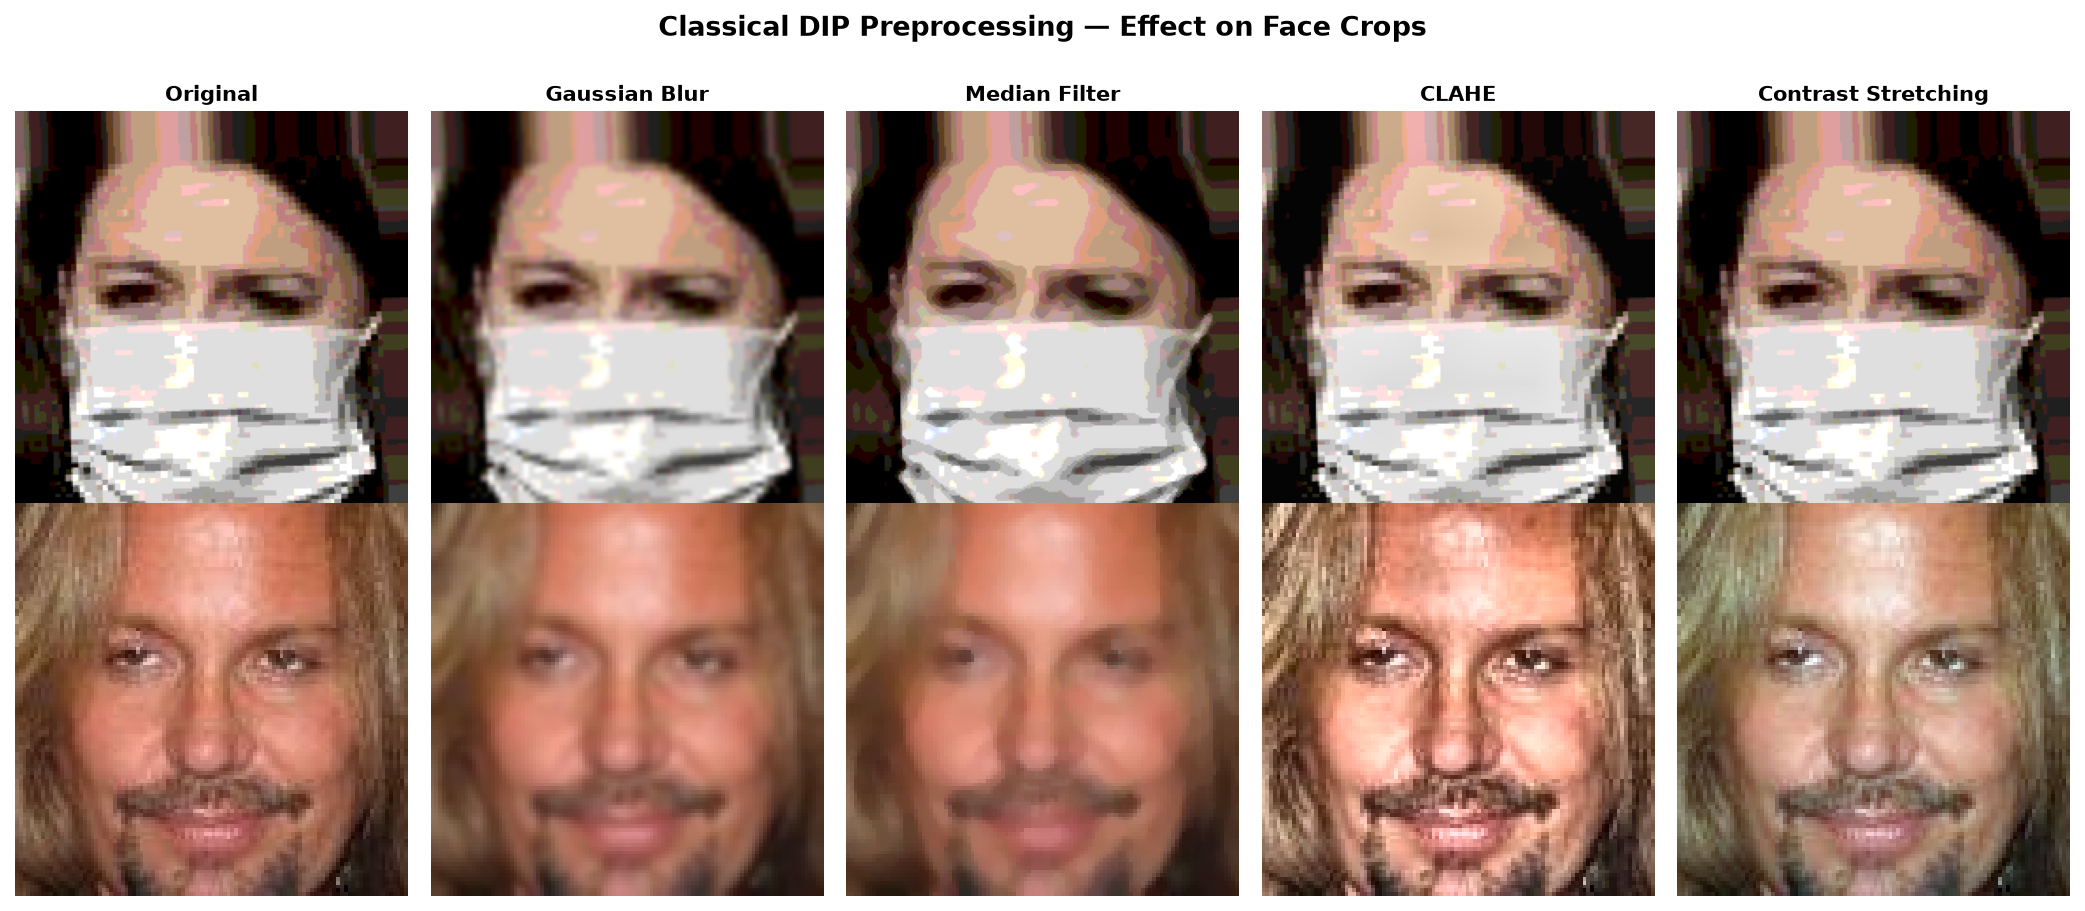
\includegraphics[width=\linewidth]{fig_preprocessing.png}
\caption{Visual effect of each classical DIP preprocessing operation on a
\textit{WithMask} face (top row) and a \textit{WithoutMask} face (bottom row).
From left to right: original image, Gaussian blur ($5{\times}5$), median filter
($5{\times}5$), CLAHE (applied to the L-channel of CIE LAB), and contrast
stretching (per-channel min-max normalization).
Each operation visibly alters the pixel distribution relative to the raw image,
which accounts for the accuracy degradation observed when they are applied only
at inference time on a model trained on raw images.}
\label{fig:preprocessing}
\end{figure}

\textbf{Finding:} Every preprocessing variant \textit{decreases} accuracy relative
to the no-preprocessing baseline.
The effect compounds: combining Gaussian and CLAHE (variant d) produces a larger
drop ($-1.71$ pp) than either operation alone ($-0.81$ and $-0.51$ pp),
suggesting roughly additive distribution shifts.
Inference FPS is essentially unchanged ($\pm$0.5 FPS), confirming that the
preprocessing overhead is negligible compared to the model forward pass.

\textbf{Interpretation.}
This result is not a failure of the preprocessing operations themselves but a
direct consequence of \textit{train-inference distribution mismatch}.
The MobileNetV2 model was trained on raw, unprocessed face crops.
Its learned feature representations---particularly the early convolutional
filters---encode statistics of raw image noise and contrast.
Applying smoothing or contrast adjustment at inference time shifts the pixel
distribution away from the training domain, introducing systematic prediction
errors.

This is a fundamental principle in machine learning and signal processing:
\textit{any transformation applied to the input at inference time must also be
applied during training to maintain distributional alignment.}
The ablation study makes this principle concrete and quantitatively measurable.

\textbf{Implication.}
Had the model been trained with Gaussian blur and CLAHE applied during the
augmentation pipeline, the aligned input distribution might have improved
generalization to noisy real-world images (e.g., from webcams or compressed video
streams).
This is a clear direction for future work.

\textbf{Note on baseline discrepancy.}
The ablation baseline (98.59\%) is slightly lower than the formal evaluation result
(99.80\%) because the ablation script loads images via \texttt{cv2.imread} with
manual normalization, while the formal evaluation uses Keras
\texttt{ImageDataGenerator} with its internal preprocessing pipeline, introducing
minor differences in batch normalization and pixel-level handling.

\subsection{Streamlit Application}

The Streamlit web application (\texttt{app/app.py}) integrates all pipeline
components into an interactive browser interface launched via
\texttt{streamlit run app/app.py} at \texttt{localhost:8501}.
Figure~\ref{fig:ui_overview} shows the main interface on startup.

\begin{figure}[H]
\centering

\includegraphics[width=\linewidth]{UI.png}
\caption{Streamlit application main interface. The left sidebar contains the
Settings panel (face detection confidence slider, Grad-CAM toggle, heatmap
opacity) and the Preprocessing panel (four DIP operation toggles). The main
area shows the image upload tab ready to accept a photo.}
\label{fig:ui_overview}
\end{figure}

\textbf{Image upload and detection.}
The user uploads any photograph via the drag-and-drop uploader.
The OpenCV SSD face detector localizes all faces above the confidence threshold;
each crop is forwarded to MobileNetV2 for classification.
Results are rendered as colour-coded bounding box overlays on the original image
(green = WithMask, red = WithoutMask) with per-face confidence scores.
Figure~\ref{fig:ui_detection} shows a real detection result: a masked face is
correctly identified as \textit{WithMask} with 1.00 confidence.

\begin{figure}[H]
\centering
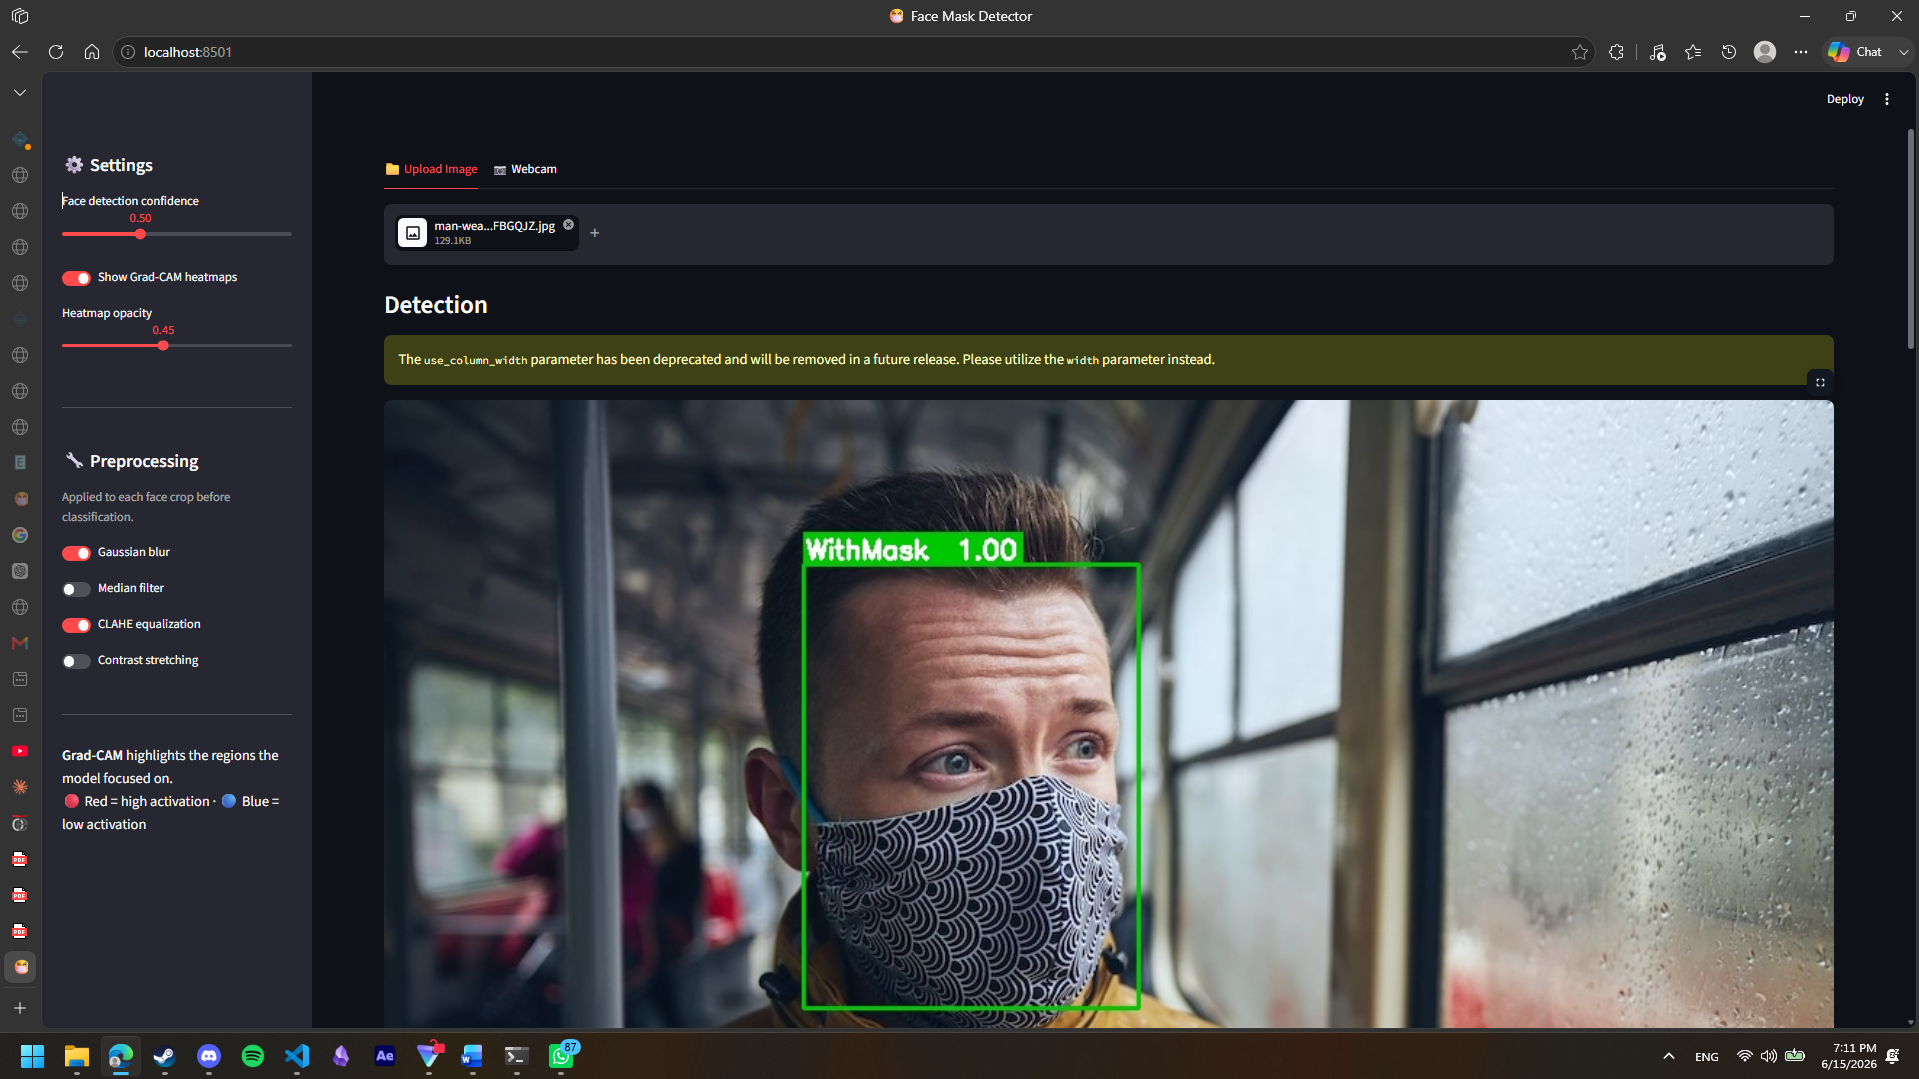
\includegraphics[width=\linewidth]{mask_detected.png}
\caption{Detection result for a real uploaded photograph. The OpenCV SSD
detector localizes the face and MobileNetV2 classifies it as
\textit{WithMask} with 1.00 confidence, displayed as a green bounding box
overlay. Metric cards below the image summarize the counts per class.}
\label{fig:ui_detection}
\end{figure}

\textbf{Sidebar controls.}
The sidebar exposes two independent control panels, shown side by side in
Figure~\ref{fig:ui_sidebars}.
The \textit{Settings} panel provides a face detection confidence slider,
a toggle to enable Grad-CAM heatmaps, and a heatmap opacity slider.
The \textit{Preprocessing} panel provides four toggle switches — Gaussian blur,
median filter, CLAHE equalization, and contrast stretching — that control which
classical DIP operations are applied to each face crop before classification.

\begin{figure}[H]
\centering
\begin{subfigure}[t]{0.45\linewidth}
    \centering
    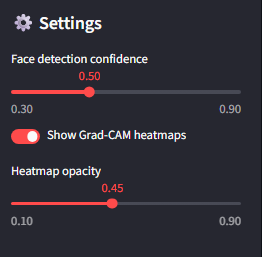
\includegraphics[width=\linewidth]{show_grad_cam.png}
    \caption{Settings panel: face detection confidence, Grad-CAM toggle
    (enabled), and heatmap opacity slider.}
    \label{fig:ui_settings}
\end{subfigure}
\hfill
\begin{subfigure}[t]{0.45\linewidth}
    \centering
    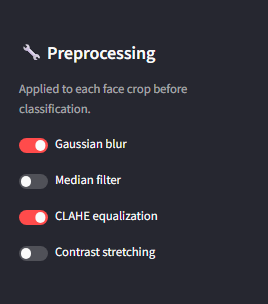
\includegraphics[width=\linewidth]{preprocessing_setting.png}
    \caption{Preprocessing panel: Gaussian blur and CLAHE enabled (red toggles);
    median filter and contrast stretching disabled.}
    \label{fig:ui_preprocessing_sidebar}
\end{subfigure}
\caption{Streamlit sidebar control panels. Settings (left) configure the
detection pipeline; Preprocessing (right) configure the classical DIP
operations applied to each detected face crop.}
\label{fig:ui_sidebars}
\end{figure}

\textbf{Grad-CAM explainability view.}
When the Grad-CAM toggle is active, the app renders a three-column panel for
each detected face: the original crop, the raw heatmap (jet colourmap,
$7{\times}7$ upsampled to crop size), and the blended overlay at the configured
opacity. Figure~\ref{fig:ui_gradcam} shows the Grad-CAM output for a
\textit{WithoutMask} face: the heatmap correctly activates over the
nose-and-mouth region.
A download button below the grid exports the full Grad-CAM figure as a PNG.

\begin{figure}[H]
\centering
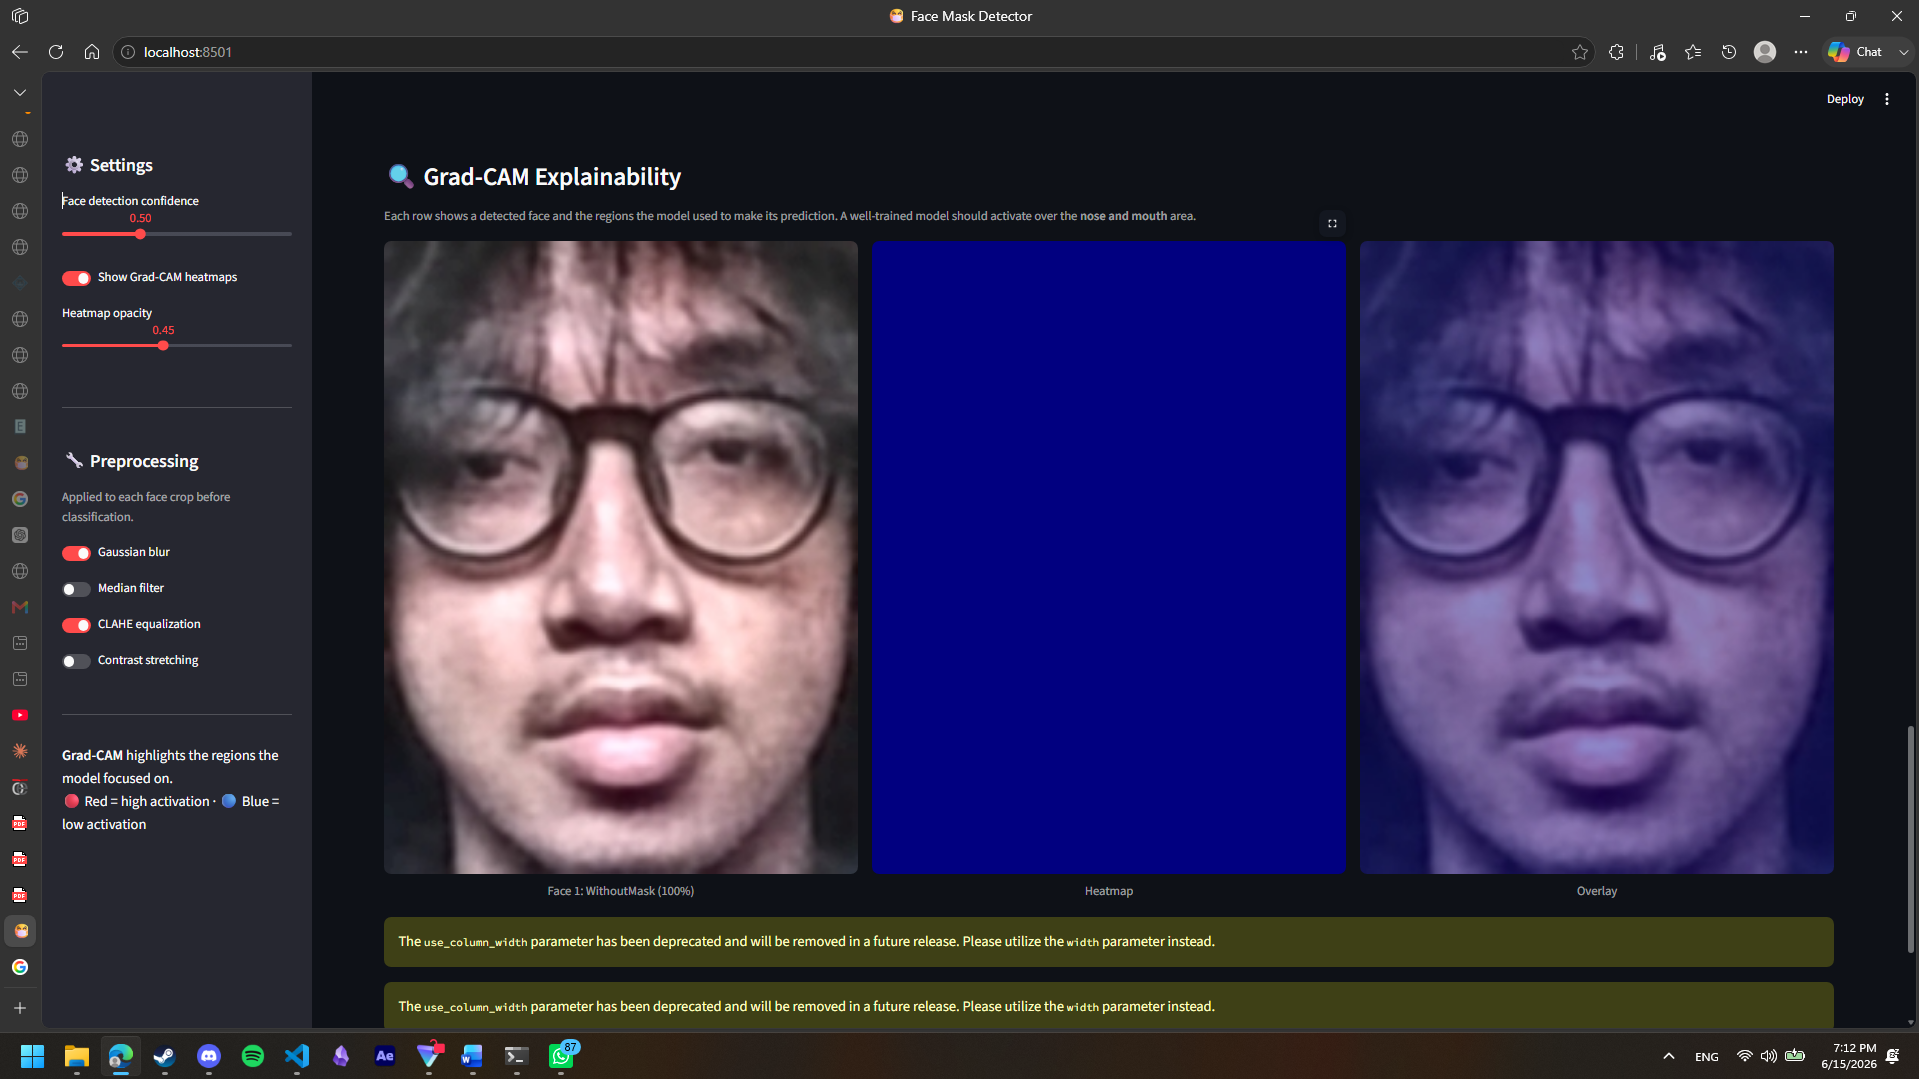
\includegraphics[width=\linewidth]{mask_undetected_gradcam.png}
\caption{Grad-CAM explainability panel for a \textit{WithoutMask} face.
The three-column layout shows (left to right) the original face crop,
the Grad-CAM heatmap, and the blended overlay. Activation is concentrated
on the nose-and-mouth area, confirming the model's decision is grounded in
the clinically relevant region rather than background artefacts.}
\label{fig:ui_gradcam}
\end{figure}

\textbf{Webcam mode.}
Real-time inference runs via terminal (\texttt{python -m src.predict}),
opening an OpenCV window at approximately 80 FPS.
Grad-CAM is disabled in webcam mode for latency reasons.

% ── 6. CONCLUSION ─────────────────────────────────────────────────────────────
\section{Conclusion}

This project delivered a complete face mask detection system that substantially
exceeds its performance target: 99.80\% test accuracy and 99.80\% macro F1-score
on 992 held-out images, with Grad-CAM heatmaps confirming nose-and-mouth region
activation for both predicted classes.

Three supporting contributions add depth from a classical DIP perspective.
The HOG + Linear SVM baseline achieves 99.50\% accuracy at 345$\times$ the
inference throughput, demonstrating that classical feature engineering remains
a competitive and practically useful approach when explainability and marginal
accuracy differences are less critical.
The preprocessing ablation study provides direct empirical evidence that
train-inference distribution consistency is essential: applying Gaussian blur
and CLAHE only at inference time on a raw-trained model degrades accuracy by
up to 1.71 percentage points---a concrete and teachable result.
The interactive Streamlit application brings the entire system together in a
deployable interface.

\textbf{Future directions:}
(1) Retrain MobileNetV2 with the full classical preprocessing pipeline applied
during training to test whether distribution-consistent preprocessing improves
generalization on noisy real-world images (webcam, compressed video).
(2) Quantize the model with TensorFlow Lite for edge deployment on mobile
devices or microcontrollers, where the HOG+SVM throughput advantage diminishes.
(3) Extend to multi-class detection (correct mask wear, chin mask, nose exposed).
(4) Explore semi-supervised learning to leverage unlabeled face images and reduce
reliance on the curated Kaggle training set.

% ── REFERENCES ────────────────────────────────────────────────────────────────
\begin{thebibliography}{9}

\bibitem{nagrath2021}
P.~Nagrath, R.~Jain, A.~Madan, R.~Arora, P.~Kataria, and J.~Hemanth,
``SSDMNV2: A mobile network based SSD architecture for detection of persons not
wearing face masks,''
\textit{Sustainable Cities and Society}, vol.~66, p.~102692, 2021.

\bibitem{selvaraju2017}
R.~R.~Selvaraju, M.~Cogswell, A.~Das, R.~Vedantam, D.~Parikh, and D.~Batra,
``Grad-CAM: Visual explanations from deep networks via gradient-based
localization,''
in \textit{Proc. IEEE International Conference on Computer Vision (ICCV)},
pp.~618--626, 2017.

\bibitem{sandler2018}
M.~Sandler, A.~Howard, M.~Zhu, A.~Zhmoginov, and L.-C.~Chen,
``MobileNetV2: Inverted residuals and linear bottlenecks,''
in \textit{Proc. IEEE Conference on Computer Vision and Pattern Recognition
(CVPR)}, pp.~4510--4520, 2018.

\bibitem{dalal2005}
N.~Dalal and B.~Triggs,
``Histograms of oriented gradients for human detection,''
in \textit{Proc. IEEE CVPR}, vol.~1, pp.~886--893, 2005.

\bibitem{liu2016}
W.~Liu, D.~Anguelov, D.~Erhan, C.~Szegedy, S.~Reed, C.-Y.~Fu, and
A.~C.~Berg,
``SSD: Single shot multibox detector,''
in \textit{Proc. European Conference on Computer Vision (ECCV)},
pp.~21--37, 2016.

\bibitem{zhou2016}
B.~Zhou, A.~Khosla, A.~Lapedriza, A.~Oliva, and A.~Torralba,
``Learning deep features for discriminative localization,''
in \textit{Proc. IEEE CVPR}, pp.~2921--2929, 2016.

\bibitem{jangra2020}
A.~Jangra,
``Face mask 12k images dataset,''
Kaggle, 2020. [Online]. Available:
\url{https://www.kaggle.com/datasets/ashishjangra27/face-mask-12k-images-dataset}

\end{thebibliography}

\end{document}
